\chapter{Infraestructura}\label{cap.infraestructura}
Este capítulo se ocupa de detallar  los componentes y piezas software existentes en las que nos hemos apoyado en el desarrollo del trabajo. Profundizaremos en las plataformas sobre las que se apoya el trabajo (ROS y JdeRobot), en la simulación de las acciones del robot que realiza Gazebo, en las librerías de mayor importancia (OpenCV para la primera práctica y PyQt para las interfaces gráficas) y, por último, en el proyecto Jupyter.

\section{Simulador Gazebo}
Gazebo\footnote{\url{http://gazebosim.org/}} es un simulador usado en robótica que permite emular diversos escenarios tridimensionales para robots autónomos (Figura 3.1). Es particularmente adecuado para probar algoritmos de elusión de objetos y de visión artificial. Cuando se trata de escribir el código que controlará un robot, especialmente si se está aprendiendo, es necesario realizar pruebas con el software, las cuales pueden ser muy costosas de implementarse en hardware real. Por ello, usamos simuladores que nos permitan comprobar en hardware virtual el comportamiento de nuestra lógica en todo momento, agilizando el desarrollo y abaratando costes. 

El simulador utilizado en este TFG será Gazebo, el cual es de código abierto. Por su versatilidad (es capaz de simular robots, objetos y sensores en entornos complejos de interior y exterior), su interfaz de gran calidad, y su robusto motor de físicas (para describir componentes como la masa del robot, rozamiento, inercia, amortiguamiento, etc.), fue elegido para realizar el DARPA Robotics Challenge (2012–2015) y está mantenido por la Fundación Open Robotics\footnote{\url{https://www.openrobotics.org/}}.

\begin{figure}[H]
  \begin{center}
    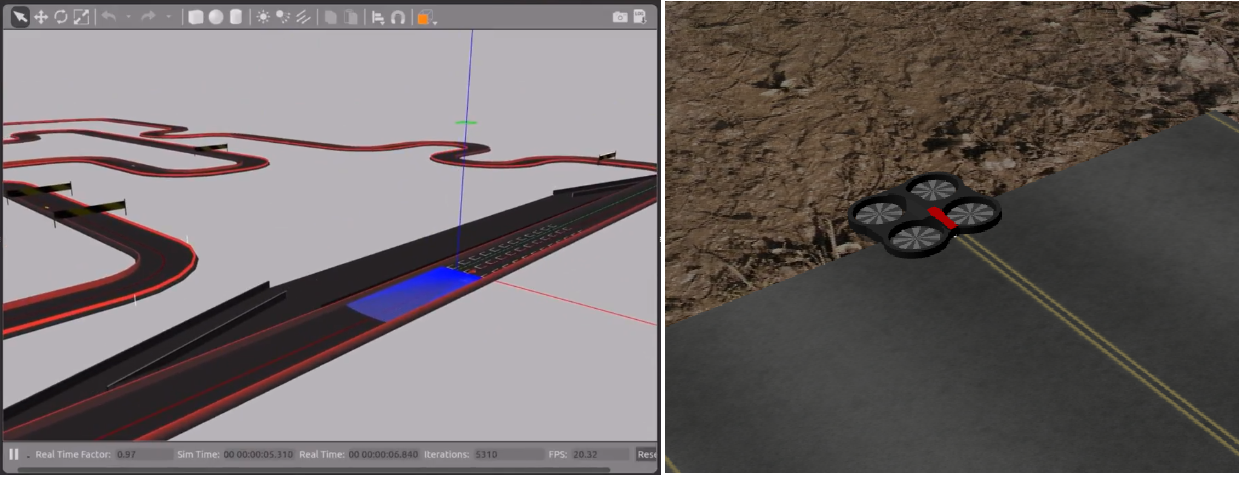
\includegraphics[width=0.9\linewidth]{figures/gazeboworlds.png}
		\caption{Ejemplo de mundo y modelo de Gazebo}
		\label{fig.worlds}
		\end{center}
\end{figure}

Los mundos 3D simulados con Gazebo se describen en ficheros con extensión “.world”, que no son más que ficheros XML (Extensible Markup Language) de descripción de documentos, definidos en el lenguaje Simulation Description Format (SDF), donde se recogen todos los elementos del escenario:

\begin{itemize}
	\item Escena: Luz ambiente, propiedades del cielo, sombras, etc.
	\item Mundo: Representa el mundo como un conjunto de modelos, \textit{plugins} y propiedades físicas.
	\item Modelo: Articulaciones, objetos de colisión, sensores, etc.
	\item Físicas: Gravedad, motor físico, paso del tiempo, colisiones, inercias, etc.
	\item \textit{Plugins}: Sobre un mundo, modelo o sensor. Pueden crearse o utilizarse los disponibles en la red como \textit{libroombaplugin.so}, que da acceso y control sobre todas las interfaces de programación de un cierto modelo de robot.
\end{itemize}

Todos y cada uno de ellos cuentan con una etiqueta propia. Los modelos de robots que se emplean en la simulación son creados mediante programas de diseño y modelado 3D como Blender o Sketchup. En la versión 7 de Gazebo se ha incorporado un editor de modelos muy básico con el que se pueden crear robots y mundos básicos. A partir del modelo, se ha de asociar un \textit{plugin} al mismo para recoger y publicar la información de los sensores, y para acceder a los actuadores y dotar al robot de inteligencia e interacción.

\section{Entorno ROS}
ROS (Robot Operating System) proporciona bibliotecas y herramientas para ayudar a los desarrolladores de software a crear aplicaciones de robots. Proporciona abstracción de hardware, controladores de dispositivo, bibliotecas, visualizadores, intercambio de mensajes y administración de paquetes entre otras cosas. Se distribuye bajo una licencia BSD de código abierto.

Uno de sus puntos fuertes es su integración con el simulador Gazebo a través de una serie de paquetes llamados \textit{gazebo\_ros\_pkgs}\footnote{\url{http://ros.org/wiki/gazebo\_ros\_pkgs}} que proporcionan las interfaces necesarias para simular un robot en Gazebo usando \textit{ROS Messages}, servicios y reconfiguración dinámica.

Este entorno se basa en la organización de una aplicación robótica como una colección de nodos, procesos que conllevan computación. Los nodos se combinan en un gráfico y se comunican entre sí mediante \textit{topics} de transmisión, servicios RPC y el Servidor de Parámetros. Un sistema de control de un robot generalmente comprenderá muchos nodos, por ejemplo, un nodo controla un láser de largo alcance, otro nodo controla los motores de las ruedas, otro se encarga de la localización, se usa otro nodo para la planificación de rutas, un nuevo nodo proporciona una vista gráfica del sistema, y así sucesivamente. El uso de nodos en ROS proporciona varios beneficios para el sistema en general. Hay tolerancia adicional a fallos ya que los problemas están aislados en nodos individuales. La complejidad del código se reduce en comparación con los sistemas monolíticos.

En cuanto a los \textit{topics} como forma de comunicación, se definen como buses sobre los cuales los nodos intercambian mensajes. Los \textit{topics} tienen una semántica de publicación y/o suscripción anónima, que desacopla la producción de información de su consumo. En general, los nodos no saben con quién o quiénes se están comunicando. En cambio, los nodos que están interesados en ciertos datos se suscriben al \textit{topic} relevante y por su parte aquellos nodos que generan datos de cierto tipo los publicarán en el \textit{topic} correspondiente. Puede haber varios editores y suscriptores de un \textit{topic}.

Dada la compatibilidad entre el entorno ROS, el simulador Gazebo y la plataforma JdeRobot, se puede hacer uso de \textit{plugins} de ROS para las simulaciones que se comunicarán con el nodo académico de cada práctica a través de \textit{topics}, por los que circulará información con el formato correspondiente. 

Existe una gran variedad de \textit{drivers} en la red para controlar las interfaces de muchos modelos, sensores y actuadores. Entre ellos, el \textit{driver usb\_cam} permite interactuar con cámaras USB estándar (por ejemplo, SonyEvi d100p o Logitech Quickcam) utilizando libusb\_cam\footnote{\url{https://github.com/libusb/libusb/wiki}}, una biblioteca multiplataforma para acceso genérico a dispositivos USB, y publica imágenes bajo el formato de mensajes \textit{sensor\_msgs::Image}\footnote{\url{http://docs.ros.org/api/sensor\_msgs/html/msg/Image.html}} 
 de ROS. Además, utiliza la biblioteca \textit{image\_transport}\footnote{\url{http://wiki.ros.org/image\_transport}} para permitir el transporte de imágenes comprimidas. A través de él obtendremos las imágenes que proporciona la cámara en la primera de las prácticas que se va a crear. Otros ejemplos son \textit{libgazebo\_ros\_laser} o \textit{libgazebo\_ros\_diff\_drive} pueden utilizarse para controlar las interfaces láser y motores respectivamente en un robot simulado.

\section{Entorno JdeRobot}
JdeRobot\footnote{\url{https://jderobot.org/}} es un \textit{middleware} abierto para el desarrollo de aplicaciones con robots y visión artificial. Esta plataforma fue creada por el Grupo de Robótica de la Universidad Rey Juan Carlos en 2003 y está licenciada como GPLv3\footnote{\url{https://www.gnu.org/licenses/quick-guide-gplv3.html}}.
Su estructura ha sido desarrollada en C y C++, aunque algunas de sus componentes están escritas Python y JavaScript. El entorno que ofrece está basado en componentes, los cuales se ejecutan como procesos. Dichos componentes interoperan entre sí a través de \textit{middlewares} de comunicaciones ICE o  ROS, según sea la aplicación. Tanto ICE como \textit{ROS-Messages} permiten la interoperación entre los componentes incluso estando desarrollados en diferentes lenguajes.

La plataforma facilita los \textit{drivers} necesarios para poner en marcha los modelos disponibles. Estos \textit{drivers} están asociados a un dispositivo hardware del robot, ya sea sensor o actuador, e incluyen el correspondiente interfaz para acceder a él. Esto simplifica el acceso desde las aplicaciones a los diferentes componentes hardware, ya que con una simple función se puede enviar o recibir datos de ellos a través de interfaces ICE o ROS.

JdeRobot ofrece soporte a una amplia gama de dispositivos entre los que podemos encontrar cuadricópteros (AR Drone de Parrot), el robot Kobuki de Yujin Robot, el humanoide NAO de Aldebaran Robotics, cámaras firewire, USB e IP, los escáneres laser LMS de SICK y URG de Hokuyo, los simuladores Stage y Gazebo, sensores de profundidad como Kinect y otros dispositivos X10 de domótica. También incluye \textit{drivers} específicos para control de cámaras y drones entre otros. Destaca para este trabajo el \textit{driver EVIcam}, de utilidad para la primera de las prácticas que se va a incluir en el entorno, que ha sido desarrollado e incluido en la plataforma JdeRobot para teleoperar cámaras vía software a través de una conexión USB. En concreto, utiliza una interfaz ICE para poder controlarla a través de comandos de movimiento. 
El código fuente puede encontrarse en: 

\url{https://github.com/JdeRobot/JdeRobot/tree/master/src/drivers/evicam_driver}

En las aplicaciones en JdeRobot se utilizan bibliotecas de software libre que son estándares de facto en su campo como OpenCV para visión, PCL para manejo de nubes de puntos o Eigen para álgebra. JdeRobot es compatible con ROS, en particular con la versión ROS-Kinetic, por lo que las aplicaciones pueden incorporar fluidamente nodos de ROS y conectarse a ellos.

Las prácticas que componen este trabajo se harán a través de la versión 5.6.1, última versión estable de la misma.

\section{Lenguaje Python}
Python\footnote{\url{https://www.python.org/}} es un lenguaje de programación interpretado, orientado a objetos y de alto nivel con semántica dinámica. Suele destacar por su apariencia intuitiva, resultando en un lenguaje fácil de aprender. Su creador fue Guido van Rossum, un investigador holandés que trabajaba en el centro de investigación CWI (Centrum Wiskunde \& Informatica). La primera versión surgió en 1991 pero no fue publicado hasta tres años después. Guido dio el nombre de Python a su lenguaje en honor a la serie de televisión \textit{Monty Python’s Flying Circus}.

Sus estructuras de datos integradas de alto nivel, combinadas con el tipado dinámico y el enlace dinámico, lo hacen muy atractivo para el desarrollo rápido de aplicaciones, también para usarlo como scripting o como lenguaje para conectar componentes existentes. La sintaxis simple y fácil de aprender de Python enfatiza la legibilidad y, por lo tanto, reduce el costo del mantenimiento del programa. Python admite módulos y paquetes, lo que fomenta la modularidad del programa y la reutilización de código. 

El intérprete de Python y la extensa biblioteca estándar están disponibles en formato fuente o binario sin cargo para las plataformas principales, y se pueden distribuir libremente.

La última versión ofrecida por Python Software Foundation, su administrador, es la 3.6.5. En este TFG vamos a emplear el lenguaje en su versión 2.7.12 junto con JdeRobot 5.6.1, que a su vez utiliza dicha versión por compatibilidad con ROS Kinetic. Usaremos este lenguaje para programar tanto los nodos académicos como las soluciones de referencia.

\section{Biblioteca OpenCV}
OpenCV\footnote{\url{https://opencv.org/}} es una librería de código abierto desarrollada inicialmente por Intel y publicada bajo licencia de BSD. Esta librería implementa gran variedad de herramientas para el procesado de imagen y el aprendizaje máquina. Sus siglas provienen del inglés, y significan \textit{“Open Source Computer Vision Library”}. Su propósito es facilitar la programación de aplicaciones de visión por computador en tiempo real.

Esta librería puede ser usada en MacOS, Windows, Android y Linux, y existen versiones para C\#, Python y Java, a pesar de que originalmente era una librería en C/C++. Además, hay interfaces en desarrollo para Ruby, Matlab y otros lenguajes.
OpenCV principalmente implementa algoritmos para las técnicas de calibración, detección de rasgos, seguimiento de caras, rastreo de objetos, análisis de la forma, análisis del movimiento, reconstrucción 3D, segmentación de objetos, reconocimiento, clasificación de acciones humanas en vídeos,…  Los algoritmos se basan en estructuras de datos flexibles acopladas con estructuras IPL (\textit{Intel Image Processing Library}), aprovechándose de la arquitectura de Intel en la optimización de la mayoría del paquete. También aprovecha la aceleración de cómputo al poder usar tarjetas gráficas avanzadas (GPUs). Fue diseñado para tener una alta eficiencia computacional. Está escrito en C y puede aprovechar las ventajas de los procesadores \textit{multicore}. Tantas son las ventajas y las posibilidades grandes compañías como Google, Yahoo, Microsoft, Intel, IBM, Sony, Honda o Toyota emplean la librería, que se ha convertido en el estándar de facto en el campo. 

En este trabajo se ha empleado la versión 3.2 de OpenCV en Python. Esta librería se empleará para todo lo relacionado con el tratamiento de imágenes (análisis y procesado). 

\section{Biblioteca PyQt}
PyQt\footnote{\url{https://pypi.org/project/PyQt5/}} es un conjunto de enlaces Python para el conjunto de herramientas Qt, un \textit{framework} multiplataforma orientado a objetos en C++  que permite desarrollar interfaces gráficas e incluye sockets, hilos, Unicode, bases de datos SQL, etc. PyQt combina todas las ventajas de Qt y Python, permite emplear todas las funcionalidades ofrecidas por Qt con un lenguaje de programación tan sencillo como Python. Fue desarrollado por Riverbank Computing Ltd y es soportado por Windows, Linux, Mac OS/X, iOS y Android.

En este proyecto se ha empleado la versión 5 de PyQt. PyQt5 es un conjunto de enlaces Python para Qt5, disponible en Python 2.x y 3.x. Tiene más de 620 clases y 6000 funciones y métodos. PyQt5 dispone de una licencia dual, es decir, los desarrolladores pueden elegir entre una licencia GPL (General Public Licence) o una licencia comercial. 
Las clases de PyQt5 se dividen en ciertos módulos, tales como QtCore, QtGui, QtWidgets, QtXml o QtSql. En las prácticas desarrolladas se ha hecho uso de los siguientes módulos para implementar las interfaces de usuario:

\begin{itemize}
	\item QtCore: contiene las funcionalidades principales no relacionadas con la interfaz gráfica. Este módulo se emplea para trabajar con archivos, diferentes tipos de datos, hilos, procesos, url, etc.
	\item QtGui: contiene clases para el desarrollo de ventanas, gráficos 2D, imágenes y texto.
	\item QtWidgets: dispone de clases que proporcionan un conjunto de elementos de interfaz de usuario para crear interfaces de usuario clásicas de escritorio. 
\end{itemize}

\section{IPython 3.0 - Jupyter}
Jupyter Notebook\footnote{\url{http://jupyter.org/}} es una aplicación web de código abierto que permite al usuario crear y compartir documentos que contengan códigos empotrados, ecuaciones, visualizaciones y textos narrativos. Entre sus usos destacan: limpieza y transformación de datos, simulación numérica, modelado estadístico, visualización de datos, aprendizaje automático, aunque su funcionalidad es mucho mayor. Jupyter es el nombre que desde hace poco se usa para referirse a IPython 3.0.

La herramienta principal de la aplicación son sus cuadernillos (\textit{Notebooks}), que son los documentos producidos por Jupyter Notebook que contienen código de computadora (por ejemplo, Python), elementos de texto enriquecido (párrafos, ecuaciones, figuras, enlaces, etc.) y demás. Los documentos del cuaderno son documentos legibles por humanos que contienen la descripción del análisis y los resultados (figuras, tablas, etc.) así como documentos ejecutables para realizar análisis de datos.
Los \textit{Notebooks} consisten en una secuencia lineal de celdas. Hay cuatro tipos básicos:

\begin{itemize}
	\item \textbf{Celdas de código}: entrada y salida del código en vivo que se ejecuta en el kernel. 
	\item \textbf{Casillas de reducción}: texto narrativo con ecuaciones LaTeX incrustadas.
	\item \textbf{Encabezado de celdas}: 6 niveles de organización jerárquica y formato.
	\item \textbf{Celdas sin formato}: texto sin formato que se incluye, sin modificaciones, cuando los cuadernillos se convierten a diferentes formatos mediante \textit{nbconvert}.
\end{itemize}

Así, la aplicación servidor-cliente permite editar y ejecutar estos \textit{Notebooks} a través de un navegador web. La aplicación Jupyter Notebook se puede ejecutar en un escritorio local que no requiere acceso a Internet o puede instalarse en un servidor remoto y acceder a ella a través de Internet. Además de mostrar, editar y ejecutar documentos, la aplicación tiene un \textit{Dashboard} (Panel de instrumentos del cuadernillo), que es similar a un ``panel de control'' que muestra los archivos locales y permite abrir documentos del cuaderno o cerrar sus núcleos (\textit{kernels}). 

Estos \textit{kernels} son ``motores computacionales'' que ejecutan el código contenido en un \textit{Notebook} (el núcleo IPython ejecuta el código Python). Existen núcleos o \textit{kernels} oficiales para muchos lenguajes (Python, Julia, R, Ruby Haskell, Scala,…), e incluso versiones distintas de un mismo lenguaje de programación. Cuando se abre un \textit{Notebook}, el \textit{kernel} asociado se inicia automáticamente, de manera que al ejecutar cada celdilla con código, realiza el cálculo y produce los resultados.  Dependiendo del tipo de cálculos, el \textit{kernel} puede consumir CPU y RAM significativas, pudiendo ejecutar procesos más exigentes. 

Estos documentos pueden ser salvados y almacenados en el sistema de ficheros local, como un documento con extensión \textit{.ipynb}, para ser ejecutado cuando se quiera. Esto nos permitirá realizar una versión análoga a la que se hará en JdeRobot a través de Jupyter, con el código de la práctica empotrado, widgets interactivos y una pequeña guía para el alumno. Los \textit{Notebooks} que haremos se basarán en código Python versión 2.7. 